\documentclass[10pt,a4paper]{article}
\usepackage[margin=2.2cm]{geometry}
\usepackage{graphicx}
\usepackage{booktabs}
\usepackage{siunitx}
\usepackage{amsmath}
\usepackage{float}
\usepackage{caption}
\usepackage{tikz}
\usetikzlibrary{calc}
\usepackage[siunitx, RPvoltages]{circuitikz}
\usepackage[hidelinks]{hyperref}
\sisetup{detect-all, table-number-alignment=center}
\setlength{\emergencystretch}{2em}

\newcommand{\GainA}{0.66}
\newcommand{\CmA}{47.1}
\newcommand{\GainB}{0.90}
\newcommand{\CmB}{1.4}
\newcommand{\GainC}{0.98}
\newcommand{\CmC}{1.3}
\newcommand{\GainD}{0.98}
\newcommand{\CmD}{0.0}
\newcommand{\MeasGainHigh}{0.50}


\title{Adapter board fixes for the SAR ADC measurement\\
\large \texttt{IHP130\_ASICONE\_ADP\_QFN48\_0p5Q\_Adapter}}
\author{Ckristian Duran}
\date{\today}

\begin{document}
\maketitle

\section{Problem}
The characterization of the ADC (report \texttt{software/mso/results/sweep\_20261022}) found three
problems on the adapter board, none of them in the chip:
\begin{enumerate}
  \item \textbf{Front-end bandwidth.} The single-ended to differential converter (TI
        SBOA216~\cite{sboa216}) is built with an LMV358 (GBW about \SI{1}{MHz}, slew rate about
        \SI{1}{V/\micro s}~\cite{lmv358}). $v_p$ passes one op-amp at unity gain, $v_n$ that op-amp
        and an inverting stage with a noise gain of 2, so the two inputs of the ADC have different
        bandwidths. At \SI{650}{kHz} the amplitude at the ADC falls to \MeasGainHigh{} of its
        low-frequency value, the input common mode moves by about half of the differential signal
        at the signal frequency, and the op-amps are close to their slew limit and distort (H2 rises
        from \SI{-45}{dBc} to \SI{-24}{dBc}; the transistor-level simulation shows that the ADC itself
        rejects the common-mode ripple, so this H2 is the op-amps). The ENOB falls from 3.8 to
        3.1 bits.
  \item \textbf{No decoupling on the references.} VREFP (pin 45) and VREFN (pin 44) come from the
        other LMV358 through jumpers JP6 and JP7, with no capacitor at the chip. The capacitive DAC
        draws charge from them at every bit decision (every \SI{100}{ns}), much faster than a
        \SI{1}{MHz} op-amp can correct, so the references may move with the code. This can produce
        the bit-weight errors seen in the static test (up to \SI{8}{\percent}); the measurement
        cannot tell them apart from errors of the chip itself.
  \item \textbf{Unfiltered \SI{0.6}{V}.} The reference of the inverting stage is the divider R1/R2
        on the \SI{1.2}{V} LDO, without a capacitor. Its noise appears doubled on $v_n$ only.
\end{enumerate}

\section{Rework of the present board}
These changes use the existing footprints (SOIC-8 for U4 and U5, 1206 passives) and need no new
board.

\subsection{Replace U4 and U5 with OPA2365}
The OPA2365~\cite{opa365} is a dual op-amp with the standard pinout of the LMV358 in SOIC-8:
\SI{50}{MHz} GBW, \SI{25}{V/\micro s}, rail-to-rail input and output, \SI{2.2}{V} to \SI{5.5}{V}
supply (the board gives \SI{3.3}{V}), $\SI{4.5}{nV}/\sqrt{\si{Hz}}$. The signals of the front end
(\SIrange{0.4}{0.8}{V}) and the references are well inside its input and output ranges. With it,
both paths of the front end have bandwidths of tens of MHz, the difference between them becomes
negligible at the frequencies of interest, and the slew rate needed (\SI{0.73}{V/\micro s} at
\SI{650}{kHz}) is 30 times below the limit. Alternative: OPA2350 (\SI{38}{MHz},
\SI{22}{V/\micro s}, also SOIC-8 and rail-to-rail).

Both are unity-gain stable but drive capacitive loads: the front end drives the RC network
through \SI{47.5}{\ohm} (as now) and the reference buffers drive \SI{1}{\micro F} through
\SI{10}{\ohm} (next section). These are the usual isolation resistors for capacitive loads; check
the phase margin with the TI SPICE model of the part before the rework.

\subsection{Decouple the references}
\begin{itemize}
  \item Remove the shunts of JP6 and JP7 and solder a \SI{10}{\ohm} resistor across each header
        instead.
  \item On the chip side of each jumper (pin B, net \texttt{adc\_vrefp} or \texttt{adc\_vrefn}),
        solder \SI{1}{\micro F} and \SI{100}{nF} X7R capacitors to the nearest ground, as close to
        pins 45 and 44 as the board allows.
\end{itemize}
The capacitors supply the charge of each bit decision; the \SI{10}{\ohm} keeps the op-amp stable
and, with \SI{1.1}{\micro F}, recharges them with a time constant of \SI{11}{\micro s}. The
average current of the DAC is about \SI{1}{\micro A}, so the drop on the resistor is
\SI{10}{\micro V}, far below an LSB (\SI{25}{mV} differential). The feedback stays at the op-amp
output, so the potentiometers keep setting the same voltages.

\begin{figure}[H]\centering
\begin{circuitikz}[scale=0.82, transform shape, font=\footnotesize]
  \draw (0,1.6) node[left]{\SI{1.2}{V}} to[short, o-] (0.6,1.6) to[pR, n=pot, l_=RV1 \SI{10}{k\ohm}] (0.6,-0.4)
        node[ground]{};
  \draw (pot.wiper) -- (1.7,0.6) coordinate (W);
  \node[op amp, noinv input up, anchor=+] (U) at (W) {\scriptsize U4A};
  \draw (U.-) -- ++(-0.3,0) |- ++(0,-0.9) -| (U.out);
  \draw (U.out) to[short] ++(0.4,0) to[R, l=\SI{10}{\ohm} (across JP6)] ++(2.2,0) coordinate (X)
        to[short, *-o] ++(2.6,0) node[right, align=left]{VREFP (pin 45)};
  \draw (X) ++(0.6,0) coordinate (C1) to[C, *-, l=\SI{1}{\micro F}] ++(0,-1.4) node[ground]{};
  \draw (X) ++(2.0,0) coordinate (C2) to[C, *-, l=\SI{100}{nF}] ++(0,-1.4) node[ground]{};
\end{circuitikz}
\caption{Reference buffer after the rework (U4A: OPA2365; VREFN is the same with RV2, U4B and JP7).}
\end{figure}

\subsection{Filter the \SI{0.6}{V} reference of the inverting stage}
Solder \SI{100}{nF} across R2 (from the non-inverting input of U5B to ground). With
R1$\parallel$R2 = \SI{5}{k\ohm} the corner is at \SI{320}{Hz}, which removes the noise of the
LDO from $v_n$ and keeps it from the comparator decisions.

\subsection{Capacitors of the RC network}
C19, C20 and C21 carry the signal: they must be C0G (NP0). The dielectric of the parts on the BOM
(LCSC C541591 and C2909429) could not be confirmed; if they are X7R, replace them, because the
capacitance of X7R depends on the voltage and distorts the signal. Optionally, C19 can go from
\SI{1.2}{nF} to \SI{470}{pF} C0G: the differential pole moves from \SI{1.33}{MHz} to
\SI{3.2}{MHz} (\SI{2}{\percent} of loss at \SI{650}{kHz} instead of \SI{10}{\percent}) while the
reservoir per side (\SI{1.06}{nF}) is still 1000 times the sampling capacitance of the ADC (the
kick of a sample is below \SI{0.4}{mV}) and recovers with \SI{50}{ns}, half of the sampling time.

\subsection{Optional: matched R3 and R4}
The gain of the inverting stage is R4/R3; a mismatch makes $v_n$ larger or smaller than $v_p$ and
leaves a small common-mode ripple at all frequencies and adds to the gain and offset error of the
measurement. The ADC rejects such a ripple well, so this is a refinement, not a fix. Two \SI{0.1}{\percent} resistors of the same value,
for example \SI{2}{k\ohm}, reduce it tenfold.

\subsection{Expected result}
Figure~\ref{fig:opt} and Table~\ref{tab:opt} apply the linear model of the measurement report
(which reproduces the measured roll-off with the LMV358) to the proposed parts.
\begin{figure}[H]\centering
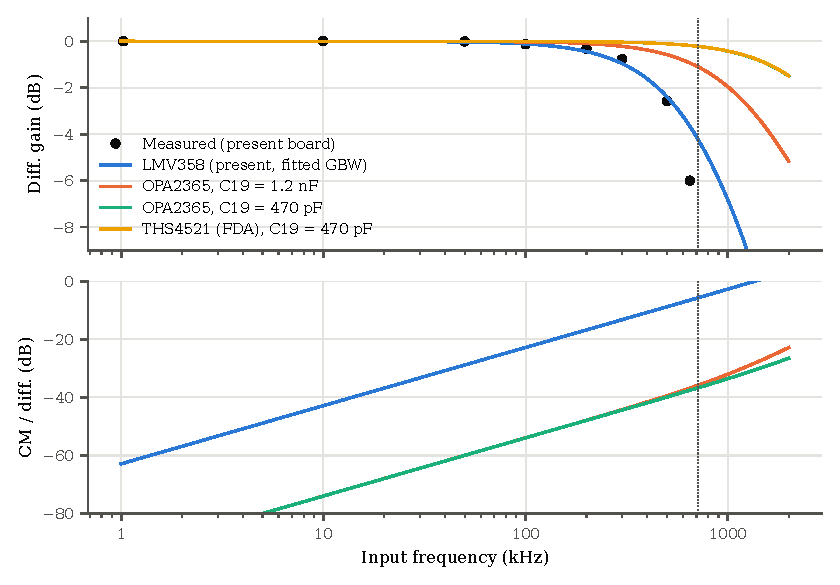
\includegraphics{build/fig/fe_options.pdf}
\caption{Differential gain and common-mode ripple at the ADC pins with the present and the proposed
front ends (model; dotted line: Nyquist frequency, \SI{714}{kHz}).}
\label{fig:opt}
\end{figure}
\begin{table}[H]\centering\small
\begin{tabular}{l S[table-format=1.2] S[table-format=1.2] S[table-format=2.2]}
\toprule
Front end & {Gain, \SI{300}{kHz}} & {Gain, \SI{650}{kHz}} & {CM/diff., \SI{650}{kHz} (\si{\percent})} \\
\midrule
LMV358 (present, fitted GBW) & 0.90 & 0.66 & 47.1 \\
OPA2365, C19 = 1.2 nF & 0.98 & 0.90 & 1.4 \\
OPA2365, C19 = 470 pF & 1.00 & 0.98 & 1.3 \\
THS4521 (FDA), C19 = 470 pF & 1.00 & 0.98 & 0.0 \\
\bottomrule
\end{tabular}

\caption{Gain relative to low frequency and common-mode ripple (model). The fully differential
amplifier has no ripple from the paths; what remains depends on its resistor matching.}
\label{tab:opt}
\end{table}
With the OPA2365 the amplitude at \SI{650}{kHz} goes from \GainA{} to \GainB{} (\GainC{} with
C19 = \SI{470}{pF}) and the common-mode ripple from \SI{\CmA}{\percent} to
\SI{\CmB}{\percent}: the front end stops limiting the sweep, and the ENOB at high frequency should
approach the low-frequency value, set by the static linearity. The reference decoupling can only be
evaluated by measurement: if the bit-weight errors of the ramp test shrink after it, they came from
the references; if not, they are in the chip.

\section{Next revision of the board}
For a new board, a fully differential amplifier is the better front end: one stage drives both
outputs through the same path, so they stay opposite at any frequency, and its output common mode
is set directly by the VOCM pin. The THS4521~\cite{ths4521} (\SI{95}{MHz} GBW,
\SI{490}{V/\micro s}, rail-to-rail output, input range including ground, \SIrange{2.5}{5.5}{V}
supply, SOIC-8 or VSSOP-8) fits the \SI{3.3}{V} supply. For the same transfer as now,
$v_d = 2(v_{in} - \SI{0.6}{V})$, use $R_f = 2 R_g$ (for example \SI{1}{k\ohm} and
\SI{499}{\ohm}), drive the gain resistor of the non-inverting input from $v_{in}$ and the other from the
decoupled \SI{0.6}{V}, and connect VOCM to the same \SI{0.6}{V}. Keep the \SI{47.5}{\ohm} resistors and the
C0G network at the ADC.

\begin{figure}[H]\centering
\begin{circuitikz}[scale=0.82, transform shape, font=\footnotesize]
  \draw (4,0) node[fd op amp, anchor=center] (F) {\scriptsize THS4521};
  \draw (F.-) to[R, l_=$R_g$ \SI{499}{\ohm}, -o] ++(-2.6,0) node[left]{\SI{0.6}{V}};
  \draw (F.+) to[R, l=$R_g$ \SI{499}{\ohm}, -o] ++(-2.6,0) node[left]{$v_{in}$};
  \draw (F.-) ++(-0.4,0) coordinate (a) to[short, *-] ++(0,1.3) to[R, l=$R_f$ \SI{1}{k\ohm}] ($(F.out +)+(0.4,1.3)$) -- ($(F.out +)+(0.4,0)$);
  \draw (F.+) ++(-0.4,0) coordinate (b) to[short, *-] ++(0,-1.3) to[R, l_=$R_f$ \SI{1}{k\ohm}] ($(F.out -)+(0.4,-1.3)$) -- ($(F.out -)+(0.4,0)$);
  \draw (F.out +) to[short, -*] ($(F.out +)+(0.4,0)$) to[R, l=\SI{47.5}{\ohm}, -o] ++(2.2,0) node[right]{$v_p$};
  \draw (F.out -) to[short, -*] ($(F.out -)+(0.4,0)$) to[R, l_=\SI{47.5}{\ohm}, -o] ++(2.2,0) node[right]{$v_n$};
  \draw (F.down) -- ++(0,-0.6) node[below]{VOCM = \SI{0.6}{V}};
\end{circuitikz}
\caption{Fully differential front end for a new board (the C0G network at the ADC as before).
$v_p - v_n = (R_f/R_g)(v_{in} - \SI{0.6}{V})$: $v_{in}$ goes to the non-inverting side so that the
positive output is in phase with it.}
\end{figure}

\section{Parts}
\begin{center}\small
\begin{tabular}{llll}
\toprule
Ref. & Change & Part & LCSC \\
\midrule
U4, U5 & LMV358 $\to$ OPA2365 & TI OPA2365AIDR, SOIC-8 & C130011 \\
       & (alternative) & TI OPA2350UA/2K5, SOIC-8 & C55904 \\
JP6, JP7 & shunt $\to$ \SI{10}{\ohm} & any 1206 \SI{1}{\percent} resistor & -- \\
new & \SI{1}{\micro F} at pins 44, 45 & Samsung CL31B105KAHNNNE, 1206 X7R \SI{25}{V} & C28322 \\
new & \SI{100}{nF} at pins 44, 45 and across R2 & as C1 on the BOM, 1206 & C697702 \\
C19--C21 & C0G if not already & 1206 C0G, \SI{50}{V}, \SI{5}{\percent} & -- \\
R3, R4 & optional, matched & RESI PTFR1206B2K00N9, \SI{2}{k\ohm} \SI{0.1}{\percent} & C2692717 \\
\midrule
new board & fully differential amplifier & TI THS4521IDR, SOIC-8 & C16092 \\
\bottomrule
\end{tabular}
\end{center}
LCSC numbers from the LCSC listings in October 2026; check stock before ordering, and confirm C28322
against the Samsung part number. LCSC marks the THS4521IDR as not recommended for new designs while
TI lists it as active.

\section{Verification}
After the rework, repeat \texttt{adc\_sweep.sh} with the same settings and rebuild the report:
\begin{itemize}
  \item the ADC amplitude should stay within a few percent of the \SI{1}{kHz} value up to
        \SI{650}{kHz}, and H2 should stay near its low-frequency level;
  \item the ENOB at high frequency should approach the low-frequency value;
  \item compare the DNL/INL of the ramp before and after the reference decoupling.
\end{itemize}

\begin{thebibliography}{9}
\bibitem{sboa216} Texas Instruments, \emph{Single-Ended Input to Differential Output Circuit},
  Analog Engineer's Circuit SBOA216B, rev.\ Oct.\ 2024. \url{https://www.ti.com/lit/pdf/sboa216}
\bibitem{lmv358} Texas Instruments, \emph{LMV321, LMV358, LMV324 Low-Voltage Rail-to-Rail Output
  Operational Amplifiers}, datasheet SLOS263Y, rev.\ Aug.\ 2023. \url{https://www.ti.com/lit/gpn/lmv358}
\bibitem{opa365} Texas Instruments, \emph{OPA365, OPA2365 50-MHz, Zer\o-Crossover, Low-Distortion,
  High CMRR, RRI/O, Single-Supply Operational Amplifiers}, datasheet SBOS365G, rev.\ May 2023.
  \url{https://www.ti.com/product/OPA2365}
\bibitem{ths4521} Texas Instruments, \emph{THS452x Very Low Power, Negative Rail Input,
  Rail-to-Rail Output, Fully Differential Amplifier}, datasheet SBOS458H, rev.\ June 2015.
  \url{https://www.ti.com/product/THS4521}
\end{thebibliography}

\end{document}
